\documentclass[a4paper,10pt]{article}
\usepackage[utf8]{inputenc}

\usepackage{tikz}
\usepackage{bbm}
\usepackage{amsmath}

\newcommand\Shifted[2]{\Delta_{#1}(#2)}
\newcommand\Scaled[2]{\otimes_{#1}(#2)}

\newcommand\SymSquare{\begin{tikzpicture}%
        \draw (0,0) -- (0,1em) -- (1em,1em) -- (1em,0) -- cycle;
\end{tikzpicture}}
\newcommand\Indicator[1]{\SymSquare(#1)}

\newcommand\SymPositiveTriangle{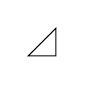
\begin{tikzpicture}%
        \draw (0,0) -- (1em,0em) -- (1em,1em) -- cycle;
\end{tikzpicture}}
\newcommand\PositiveTriangle[1]{\SymPositiveTriangle(#1)}

\newcommand\SymNegativeTriangle{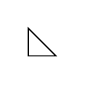
\begin{tikzpicture}%
        \draw (0,0) -- (0,1em) -- (1em,0em) -- cycle;
\end{tikzpicture}}
\newcommand\NegativeTriangle[1]{\SymNegativeTriangle(#1)}

\newcommand\Convolution{\star}
\newcommand\ConvolutionInt[2]{\int_{-\infty}^{\infty}#1 \mathrm{d}#2}

\title{Convolution formulas using shapes}
\author{Francois Gindraud}
\date{}

\begin{document}

\maketitle

Formulas for convolutions are very quickly unwieldy, especially if the functions being convoluted are defined by parts.
In this case, it is easier to use abstractions over functions shapes, and compute the convolution of two functions by using the geometry of the shape instead of raw integration.

\paragraph{Convolution}
Convolution is noted using the $\Convolution$ operator, with the usual definition:
\[ \left[ f \Convolution g \right](x) = \ConvolutionInt{f(x - t) g(t)}{t} \]
Convolution is commutative and associative.

\section{Combinators}

\paragraph{Time shifting}
The time shift combinator of shift $h$ moves the shape $f$ forward along the time axis by $h$.
For a shape $f$ \emph{centered} on $c$, $\Shifted{h}{f}$ is \emph{centered} on $c+h$.
\[ \Shifted{h}{f}(x) = f(x - h) \]
Time shifts combine additively:
\[ \Shifted{h}{\Shifted{h'}{f}}= \Shifted{h+h'}{f} \]
Convolution of shifted functions is the shift of convolutions:
\[
    \left[ \Shifted{h}{f} \Convolution g \right](x) =
    \ConvolutionInt{ f((x - t) - h) g(t) }{t} = 
    \left[ f \Convolution g \right](x-h) =
    \Shifted{h}{f \Convolution g}(x)
\]

\paragraph{Scaling}
The scaling combinator scales the shape $f$ by a factor $c$ on the vertical axis.
\[ \Scaled{c}{f}(x) = c \times f(x) \]
Scaling combines multiplicatively with itself, and can be swapped with time shift:
\[ \Scaled{c}{\Scaled{c'}{f}} = \Scaled{c \times c'}{f} \]
\[ \Scaled{c}{\Shifted{h}{f}} = \Shifted{h}{\Scaled{c}{f}} \]
Convolution of scaled functions is a scaled convolution:
\[ \Scaled{c}{f} \Convolution g = \Scaled{c}{f \Convolution g} \]

\section{Basic shape definitions}

\paragraph{Indicator function}
The \emph{indicator function} of width $l$ is a rectangle of width $l$, height $1$, horizontally centered on $0$.
\[
    \Indicator{l}(x) =
    \mathbbm{1}_{\left[ -\frac{l}{2}, \frac{l}{2} \right]}(x) =
    \begin{cases}
        1 & x \in \left[ -\frac{l}{2}, \frac{l}{2} \right] \\
        0 & \text{otherwise}
    \end{cases}
\]

\paragraph{Positive triangle}
The \emph{positive triangle} of side $c$ is a triangle formed by coordinates $\{ (0,0), (c, 0), (c,c) \}$:
\[
    \PositiveTriangle{c}(x) = \begin{cases}
        x & x \in \left[ 0, c \right] \\
        0 & \text{otherwise}
    \end{cases}
\]

\paragraph{Negative triangle}
The \emph{negative triangle} of side $c$ is a triangle formed by coordinates $\{ (0,0), (-c, 0), (-c,c) \}$:
\[
    \NegativeTriangle{c}(x) = \begin{cases}
        -x & x \in \left[ -c, 0 \right] \\
        0 & \text{otherwise}
    \end{cases}
\]

\end{document}
